\chapter{Переходим к объектам: обобщённые функции}
\label{ch:16}

\thispagestyle{empty}

Поскольку Lisp был создан за пару десятилетий до того момента, когда
объектно-ориентированное программирование (ООП) стало популярным\footnote{Язык Simula,
  который сейчас считается первым объектно-ориентированным языком, был создан в начале
  1960-х годов, лишь несколько лет после создания McCarthy первого Lisp.  Однако
  объектно-ориентированный подход не был популярен до начала 1980-х годов, когда была
  выпущена первая доступная версия Smalltalk, за которой последовал выпуск C++ несколько
  лет спустя.  Smalltalk позаимствовал часть идей из Lisp и объединил их с идеями из
  Simula, что в результате привело к появлению динамического, объектно-ориентированного
  языка, в то время как C++ комбинировал идеи Simula и Си, что породило статический
  объектно-ориентированный язык. Это первоначальное разделение привело ко множеству
  неясностей в определении того, что есть объектно-ориентированный подход.  Люди, которые
  привыкли к C++, говорят, что некоторые его аспекты, такие как строгая инкапсуляция
  данных, являются ключевыми характеристиками ООП. А люди, воспитанные на Smalltalk, в
  свою очередь, указывают, что многие возможности C++ являются лишь возможностями C++, а не
  основами ООП.  Говорят, Alan Kay, отец Smalltalk, однажды сказал: \textit{<<Я ввёл термин
    объектно-ориентированный и могу сказать, что C++~-- это не то, что я имел в виду>>.}},
начинающие Lisp-программисты иногда удивляются, открывая для себя, насколько полноценным
объектно-ориентированным языком является Common Lisp.  Непосредственные его
предшественники разрабатывались в то время, когда объектно-ориентированное
программирование было волнующе-новой парадигмой и проводилось много экспериментов на тему
включения его идей (особенно из языка Smalltalk) в Lisp.  Как часть процесса
стандартизации Common Lisp объединение идей нескольких этих экспериментов было
представлено под названием Common Lisp Object System (Объектная система Common Lisp) или
CLOS\translationnote{Читается <<see-loss>>. Источник: Norvig P. Paradigms of Artificial
  Intelligence Programming: Case Studies in Common Lisp.}. Стандарт ANSI
включил CLOS в язык, так что сейчас нет смысла говорить о CLOS как об отдельной сущности.

Возможности CLOS, внесённые в Common Lisp, варьируются от тех, без которых крайне тяжело
обойтись, до относительно эзотеричных проявлений философии Lisp как языка-инструмента для
построения языков.  Полный обзор всех возможностей лежит за пределами данной книги, но в
этой и следующей главах я опишу базовые возможности и дам обзор подхода Common Lisp к
объектам.

Вначале вы должны были заметить, что объектная система Common Lisp предлагает достаточно
отличающуюся от других языков реализацию принципов ООП. Если вы имеете глубокое понимание
фундаментальных идей, заложенных в основу ООП, то вы, вероятно, оцените способ, который
использовался в Common Lisp для их реализации.  С другой стороны, если у вас есть опыт
использования ООП только на одном языке, то подход Common Lisp может показаться вам
несколько чуждым; вы должны избегать предположений, что для языка существует только один
способ реализации принципов ООП\footnote{Есть люди, которые полностью отрицают, что Common
  Lisp является объектно-ориентированным языком.  В~частности, люди, рассматривающие
  строгую инкапсуляцию данных в качестве ключевой характеристики ООП (обычно это
  приверженцы статических языков, таких как C++, Eiffel или Java), не считают Common Lisp
  <<правильным>> объектно-ориентированным языком.  Конечно, при использовании данного
  определения Smalltalk~-- один из первых объектно-ориентированных языков~-- также не будет
  им считаться.  С другой стороны, люди, рассматривающие передачу сообщений как ключевую
  составляющую ООП, тоже не будут рады утверждению о объектной ориентированности Common
  Lisp, поскольку обобщённые функции Common Lisp предоставляют степени свободы, не
  предлагаемые чистой передачей сообщений.}.  Если у вас имеется небольшой опыт
объектно-ориентированного программирования, то вы не должны испытывать проблем с
пониманием изложенных здесь объяснений, хотя в этом случае, возможно, будет лучше
проигнорировать сравнения с подходами других языков.

\section{Обобщённые функции и классы}

Мощной и фундаментальной особенностью ООП является способ организации программ путём
определения типов данных и связывании операций с ними.  В~частности, вам может
понадобиться возможность исполнять операцию, получая поведение, определённое типом объекта
(или объектов), для которого эта операция выполняется. Классическим примером, представленным
во всех введениях в ООП, является операция рисования, применимая к объектам,
представляющим различные геометрические фигуры.  Для рисования окружностей, треугольников
или квадратов могут быть реализованы разные методы draw, которые будут отображать
окружность, треугольник или квадрат, в зависимости от объекта, к которому применяется
операция рисования. Эти реализации вводятся раздельно, и новые версии для рисования других
фигур могут быть определены, не затрагивая ни кода базового класса, ни других draw.  Эта
возможность ООП имеет красивое греческое имя \textit{<<полиморфизм (polymorphism)>>},
переводимое как <<множество форм>>, поскольку одна концептуальная операция, такая как
рисование объекта, может иметь множество различных конкретных форм.

Common Lisp, подобно другим современным объектно-ориентированным языкам, основан на
классах; все объекты являются экземплярами определённого класса\footnote{Языки, основанные
  на прототипах (prototype-based languages), являются другим видом объектно-ориентированных
  языков. В~таких языках (самым известным примером будет, пожалуй, JavaScript) объекты
  создаются путём клонирования объекта-прототипа. После клонирования объект может быть
  модифицирован и использован как прототип для других объектов.}.  Класс объекта
определяет его представление~-- встроенные классы, такие как \lstinline{NUMBER} и \lstinline{STRING},
имеют скрытое представление, доступное только через стандартные функции для работы с этими
типами, в то время как экземпляры классов, определённых пользователем, состоят из
именованных частей, называемых слотами (вы увидите это в следующей главе).

Классы образуют иерархию/классификацию всех объектов.  Класс может быть определён как
подкласс других классов, называемых базовыми (или суперклассами).  Класс наследует от
суперклассов часть своего определения, а экземпляры класса также считаются и экземплярами
суперклассов.  В~Common Lisp иерархия классов имеет один корень~-- класс \lstinline{T}, который
является прямым (или косвенным) суперклассом для всех остальных классов.  Таким образом, в
Common Lisp все данные являются экземплярами класса \lstinline{T}\footnote{\lstinline{T} является
  значением-константой, и класс \lstinline{T} не имеет никакого отношения к этой константе, за
  тем исключением, что они имеют одинаковые имена.  Значение \lstinline{T} является экземпляром
  класса \lstinline{SYMBOL} и, косвенно, экземпляром класса \lstinline{T}.}.  Common Lisp также
поддерживает множественное наследование~-- один класс может иметь несколько прямых
суперклассов.

Вне семейства языков Lisp почти все объектно-ориентированные языки следуют базовому
дизайну, заданному языком Simula, когда поведение, связанное с классом, реализуется в виде
методов или функций-членов, которые относятся к определённому классу.  В~этих языках
метод, вызываемый для определённого объекта, и класс, к которому этот объект относится,
определяют, какой код будет запущен.  Такая модель называется (в терминологии Smalltalk)
передачей сообщений (message-passing).  Концептуально вызов методов начинается с отправки
сообщения, содержащего имя запускаемого метода и необходимые аргументы, экземпляру
объекта, метод которого вызывается.  Объект затем использует свой класс для поиска метода,
связанного с именем, указанным в сообщении, и вызывает его.  Поскольку каждый класс может
иметь собственный метод для заданного имени, то одно и то же сообщение, посланное разным
объектам, может вызывать разные методы.

Ранние реализации объектной системы Lisp работали аналогичным образом, предоставляя
специальную функцию \lstinline{SEND}, которая могла быть использована для отправки сообщения
определённому объекту.  Однако это было не совсем удобно, поскольку это делало вызов
метода отличным от обычного вызова функции.  Синтаксически вызов метода записывался:

\begin{myverb}
(send object 'foo)
\end{myverb}

\noindent{}вместо

\begin{myverb}
(foo object)
\end{myverb}

Более важным являлось то, что поскольку методы не являлись функциями, то они не могли быть
переданы как аргументы для функций высшего порядка, таких как \lstinline{MAPCAR}; если кто-то
хотел вызвать метод для всех элементов списка, используя \lstinline{MAPCAR}, то он должен был
писать вот так:

\begin{myverb}
(mapcar #'(lambda (object) (send object 'foo)) objects)
\end{myverb}

\noindent{}вместо

\begin{myverb}
(mapcar #'foo objects)
\end{myverb}

В~конечном счёте люди, работавшие над объектными системами Lisp, унифицировали методы и
функции путём введения нового их вида, называемого обобщённым (generic).  В~дополнение к
решению описанных выше проблем обобщённые функции открыли новые возможности объектной
системы, включая множество таких, которые попросту не имели смысла в объектных системах с
передачей сообщений.

Обобщённые функции суть сердце объектной системы Common Lisp и тема оставшейся части
данной главы.  Несмотря на то что я не могу говорить об обобщённых функциях без
упоминания классов, сначала я остановлюсь на том, как определить и использовать обобщённые
функции.  А в следующей главе я покажу вам, как определять ваши собственные классы.

\section{Обобщённые функции и методы}

Обобщённая функция определяет абстрактную операцию, указывая имя операции и список
параметров, но не определяет реализацию.  Вот, например, как вы можете определить
обобщённую функцию \lstinline{draw}, которая будет использоваться для отрисовки различных фигур
на экране:

\begin{myverb}
(defgeneric draw (shape)
  (:documentation "Draw the given shape on the screen."))
\end{myverb}

Я опишу синтаксис \lstinline{DEFGENERIC} в следующем разделе; сейчас лишь замечу, что это
определение совсем не содержит кода.

Обобщённая функция являются таковой в том смысле, что она может (по крайней мере, в теории)
принимать в качестве аргументов любые объекты\footnote{Здесь, как и везде, под объектом
  понимается любой тип данных Lisp~-- Common Lisp не делает различия, как это делают
  некоторые языки, между объектами и <<примитивными>> типами данных; все типы данных в
  Common Lisp являются объектами, и каждый объект является экземпляром класса.}.  Однако
сама эта функция не делает ничего; если вы просто определили её, то при вызове с любыми
аргументами она будет выдавать ошибку. Действующая реализация обобщённой функции
обеспечивается методами. Каждый метод предоставляет реализацию обобщённой функции для
отдельных классов аргументов.  Вероятно, наибольшим отличием между системами с обобщёнными
функциями и системами с передачей сообщений является то, что методы не принадлежат к
классам; они относятся к обобщённой функции, которая ответственна за определение того,
какой метод (или методы) будет исполняться в ответ на конкретный вызов.

Методы указывают, какой вид аргументов они могут обрабатывать путём специализации
требуемых параметров, определённых обобщённой функцией.  Например, для обобщённой функции
\lstinline{draw} вы можете определить один метод, который определяет специализацию параметра
\lstinline{shape} для объектов, которые являются экземплярами класса \lstinline{circle}, в то время
как другой метод специализирует \lstinline{shape} для экземпляров класса \lstinline{triangle}.  Они
могут выглядеть следующим образом (не вдаваясь в подробности рисования конкретных фигур):

\begin{myverb}
(defmethod draw ((shape circle))
  ...)

(defmethod draw ((shape triangle))
  ...)
\end{myverb}

При вызове обобщённой функции она сравнивает переданные аргументы со спе\-циа\-ли\-за\-то\-ра\-ми
каждого из её методов с целью найти среди них апплицируемые~-- чьи специализаторы
совместимы с фактическими параметрами (вызова). Если вы вы\-зы\-вае\-те \lstinline{draw}, передавая
экземпляр \lstinline{circle}, то применяется метод, который специализирует \lstinline{shape} для
класса \lstinline{circle}, а если вы вызываете, передавая \lstinline{triangle}, то будет вызван
метод, который специализирует \lstinline{shape} для \lstinline{triangle}.  В~простых случаях будет
подходить только один метод, который и будет обрабатывать вызов.  В~более сложных случаях
могут быть применимы несколько методов; они будут скомбинированы, как я опишу в разделе
<<Комбинация методов>>, в один действующий метод, который обработает данный вызов.

Вы можете специализировать параметры двумя способами~-- обычно вы указываете класс,
экземпляром которого должен быть аргумент.  Поскольку экземпляры класса также
рассматриваются как экземпляры его суперклассов, то метод, специализированный для
конкретного класса, также применим для аргументов, которые могут быть как экземлярами
специализирующего класса, так и его подклассов.  Другой вид специализации~-- так
называемый \lstinline{EQL}-специализатор, который определяет конкретный объект, к которому
применим данный метод.

Когда обобщённая функция имеет только методы, специализированные для одного параметра, и
все специализации являются специализациями классов, то результат вызова обобщённой функции
сильно похож на вызов метода в системе с передачей сообщений~-- комбинация имени операции
и класса объекта, для которого она вызывается, определяет, какой метод будет вызван.

Однако изменение порядка поиска открывает новые возможности, которых нет в системах с
передачей сообщений.  Обобщённые функции поддерживают методы, которые специализируются для
множества параметров, предоставляя каркас, который делает множественное наследование более
управляемым и который позволяет вам использовать декларативные конструкции для контроля
того, как методы комбинируются в эффективный метод, поддерживая несколько общих методов
использования без наличия кучи дополнительного кода. Я опишу эти вопросы очень скоро.  Но
сначала вам необходимо взглянуть на основы использования двух макросов, которые
применяются для определения обобщённых функций: \lstinline{DEFGENERIC} и \lstinline{DEFMETHOD}.

\section{DEFGENERIC}

Чтобы дать вам почувствовать эти макросы и ознакомиться с возможностями, которые они
предоставляют, я покажу вам некоторый код, который вы могли бы написать как часть
банковского приложения или, иначе, игрушечное банковское приложение; главная задача~--
ознакомиться с возможностями языка, а не научиться писать банковское программное
обеспечение.  Например, данный код даже не пытается претендовать на работу с разными
валютами, а также оставляет в стороне вопросы аудита и целостности транзакций.

Поскольку я буду обсуждать вопросы создания новых классов только в следующей главе, сейчас
вы можете просто предположить, что определённые классы уже существуют: для начала
предположим, имеется класс \lstinline{bank-account}, и он имеет два подкласса~--
\lstinline{checking-account} и \lstinline{savings-account}.  Иерархия классов выглядит следующим
образом:

\begin{figure}[h]
  \centering
  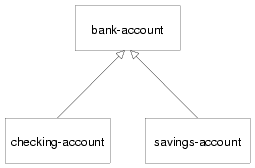
\includegraphics[scale=0.7]{images/account-hierarchy.png}
\end{figure}

Первой обобщённой функцией будет \lstinline{withdraw}, которая уменьшает баланс на указанную
сумму.  Если баланс меньше этой суммы, то она должна выдать ошибку и оставить баланс в
неизменном виде.  Вы можете начать с определения обобщённой функции при помощи
\lstinline{DEFGENERIC}.

Основная форма \lstinline{DEFGENERIC} похожа на \lstinline{DEFUN}, за тем исключением, что нет тела
функции.  Список параметров \lstinline{DEFGENERIC} определяет параметры, которые должны
приниматься всеми методами, определёнными для данной обобщённой функции.  Вместо тела
\lstinline{DEFGENERIC} может содержать различные опции.  Одной из опций, которую вы должны
всегда указывать, является \lstinline{:documentation}, которая используется для указания строки
с описанием назначения обобщённой функции.  Поскольку обобщённая функция является
полностью абстрактной, важно, чтобы и пользователь, и программист имели чёткое
представление о том, что она делает.  Таким образом, вы можете определить \lstinline{withdraw}
следующим образом:

\begin{myverb}
(defgeneric withdraw (account amount)
  (:documentation "Withdraw the specified amount from the account.
Signal an error if the current balance is less than amount."))
\end{myverb}

\section{DEFMETHOD}

Сейчас вы готовы к использованию \lstinline{DEFMETHOD} для определения методов, которые
реализуют \lstinline{withdraw}\footnote{С технической точки зрения, вы можете вообще не
  использовать \lstinline{DEFGENERIC}~-- если вы определяете метод с помощью \lstinline{DEFMETHOD} и
  соответствующая обобщённая функция не определена, она будет создана автоматически.
  Однако хорошим тоном считается явное определение обобщённой функции, поскольку это
  предоставляет хорошее место для документирования её предназначения.}.

Список параметров метода должен быть конгруэнтен его обобщённой функции.  В~данном случае
это означает, что все методы, определённые для \lstinline{withdraw}, должны иметь два
обязательных параметра.  В~более общих чертах методы должны иметь то же самое количество
обязательных и необязательных параметров и, кроме этого, должны уметь принимать любые
аргументы, относящиеся к остаточным (\lstinline!&rest!) или именованным (\lstinline!&key!)
параметрам, определённым в обобщённой функции\footnote{Метод может <<принимать>>
  именованные и остаточные аргументы, определённые в обобщённой функции, путём указания
  параметра \lstinline!&rest!, таких же именованных параметров или указания
  \lstinline!&allow-other-keys! вместе с \lstinline!&key!.  Метод также может указывать
  именованные параметры, не указанные в списке параметров обобщённой функции: когда
  вызывается обобщённая функция, будет принят любой именованный параметр, указанный
  обобщённой функцией или любым другим подходящим методом.  \textit{Одним следствием
    из правила соответствия является то, что все методы одной и той же обобщённой функции
    будут иметь совпадающие списки параметров.  Common Lisp не поддерживает перегрузку
    методов так, как это делают некоторые статически типизированные языки, как С++ и Java,
    где одно и то же имя может использоваться для методов с разными списками параметров.}
}.

Поскольку базовые действия по списанию денег со счёта являются одинаковыми для всех
счетов, то вы можете определить метод, который специализирует параметр \lstinline{account}
для класса \lstinline{bank-account}.  Вы можете предположить, что функция
\lstinline{balance} возвращает текущее значение суммы на счёте и может быть использована
вместе с функцией \lstinline{SETF} (и~таким образом вместе с \lstinline{DECF}) для
установки значения баланса.  Функция \lstinline{ERROR} является стандартной функцией для
сообщения об ошибках, и я её подробно опишу в главе~\ref{ch:19}.  Используя эти две
функции, вы можете определить основной метод \lstinline{withdraw} примерно так:

\begin{myverb}
(defmethod withdraw ((account bank-account) amount)
  (when (< (balance account) amount)
    (error "Account overdrawn."))
  (decf (balance account) amount))
\end{myverb}

Как видно из этого кода, форма \lstinline{DEFMETHOD} более похожа на \lstinline{DEFUN}, по сравнению
с \lstinline{DEFGENERIC}.  Основным отличием является то, что требуемые параметры могут быть
специализированы путём замены имени параметра на список из двух элементов.  Первым
элементом является имя параметра, а вторым~-- специализатор, который может быть либо
именем класса, либо \lstinline{EQL}-специализатором, форму которого я опишу чуть позже.  Имя
параметра может быть любым~-- оно не обязательно должно совпадать с именем, указанным в
объявлении обобщённой функции, несмотря на то что чаще всего они совпадают.

Этот метод будет использоваться тогда, когда первый аргумент \lstinline{withdraw} является
экземпляром класса \lstinline{bank-account}.  Второй параметр, \lstinline{amount}, неявно
специализируется для класса \lstinline{T}, а поскольку все объекты являются экземплярами
\lstinline{T}, это никак не затрагивает применимость метода.

Теперь предположим, что все чековые счета имеют защиту от перерасхода.  Так что каждый
чековый счёт связан с другим счётом в банке, с которого будет производиться списание,
когда на чековом счету недостаточно денег для списания.  Вы можете предположить, что
функция \lstinline{overdraft-account} получает объект класса \lstinline{checking-account} и
возвращает объект класса \lstinline{bank-account}, представляющего собой связанный счёт.

Таким образом, списание с объекта класса \lstinline{checking-account} требует выполнения
дополнительных шагов в сравнении со списанием с обычного объекта \lstinline{bank-account}.
Сначала вы должны проверить, является ли списываемая сумма большей, чем имеющаяся на
счету, и если это так, то перенести недостающую сумму со связанного счёта.  Затем вы
можете продолжать так же, как и с обычным объектом \lstinline{bank-account}.

Так что вы можете захотеть определить метод \lstinline{withdraw}, специализированный для
\lstinline{checking-account}, для обработки перевода денег с другого счёта и последующей
передачи управления методу, специализированному для \lstinline{bank-account}.  Такой метод
может выглядеть вот так:

\begin{myverb}
(defmethod withdraw ((account checking-account) amount)
  (let ((overdraft (- amount (balance account))))
    (when (plusp overdraft)
      (withdraw (overdraft-account account) overdraft)
      (incf (balance account) overdraft)))
  (call-next-method))
\end{myverb}

Функция \lstinline{CALL-NEXT-METHOD} является частью системы обобщённых функций и используется
для комбинации \textit{подходящих} методов.  Она сообщает, что контроль должен быть
передан от текущего метода к методу, специализированному для
\lstinline{bank-account}\footnote{\lstinline{CALL-NEXT-METHOD} аналогичен вызову метода для
  \lstinline{super} в Java или использованию явно указанного метода или функции класса в Python
  или C++.}.  Когда он вызывается без аргументов, как это было сделано в нашем примере,
следующий в цепочке метод будет вызван с теми же аргументами, которые были переданы
обобщённой функции.  Он также может быть вызван с явным указанием аргументов, которые
будут переданы следующему методу.

Вам не обязательно вызывать \lstinline{CALL-NEXT-METHOD} в каждом методе.  Однако если вы не
будете вызывать эту функцию, то новый метод будет полностью отвечать за реализацию
требуемого поведения обобщённой функции.  Например, если вы хотите создать подкласс
\lstinline{bank-account}, названный \lstinline{proxy-account}, который не будет отслеживать свой
баланс, а вместо этого будет делегировать списание средств другому счёту, то вы можете
записать этот метод следующим образом (предполагая, что функция \lstinline{proxied-account}
возвращает соответствующий счёт):

\begin{myverb}
(defmethod withdraw ((proxy proxy-account) amount)
  (withdraw (proxied-account proxy) amount))
\end{myverb}

В~заключение \lstinline{DEFMETHOD} также позволяет вам создавать методы, которые
специализированы для конкретного объектаk используя \lstinline{EQL}-специализатор.  Например,
предположим, что банковское приложение \textit{будет} развёрнуто в каком-то
коррумпированном банке.  Предположим, что переменная \lstinline{*account-of-bank-president*}
хранит ссылку на конкретный банковский счёт, который относится (как это видно из имени) к
президенту банка.  Также предположим, что переменная \lstinline{*bank*} представляет весь банк,
а функция \lstinline{embezzle} крадёт деньги у банка.  Президент банка может попросить вас
<<исправить>> функцию \lstinline{withdraw} таким образом, чтобы она обрабатывала его счёт
другим способом.

\begin{myverb}
(defmethod withdraw ((account (eql *account-of-bank-president*)) amount)
  (let ((overdraft (- amount (balance account))))
    (when (plusp overdraft)
      (incf (balance account) (embezzle *bank* overdraft)))
  (call-next-method)))
\end{myverb}

Однако заметьте, что форма, указанная в \lstinline{EQL}-специализаторе, который используется
для указания объекта (в нашем случае это \lstinline{*account-of-bank-president*}), вычисляется
один раз, когда вычисляется \lstinline{DEFMETHOD}.  Этот метод будет специализирован для
значения \lstinline{*account-of-bank-president*} в тот момент, когда этот метод был определён;
последующие изменения переменной не изменяют метода.

\section{Комбинирование методов}

Вне кода метода использование \lstinline{CALL-NEXT-METHOD} не имеет смысла.  Внутри метода
использование этой функции обретает смысл за счёт того, что механизмы реализации
обобщённых функций при каждом запуске создают эффективный метод из методов, для которых
применимы текущие параметры.  Идея построения эффективного метода путём комбинации
методов, для которых применимы текущие аргументы, является основой концепции обобщённых
функций, и это позволяет обобщённым функциям реа\-ли\-зо\-вы\-вать возможности, которые недоступны
в системах с передачей сообщений.  Так что следует поближе познакомиться с тем, что в
действительности происходит.  Люди, которые давно знакомы с концепциями систем с передачей
сообщений, должны обратить на данный материал особое внимание, поскольку обобщённые функции
кардинально меняют диспатчеризацию методов, по сравнению с передачей сообщений, делая
обобщённую функцию (а не класс) ответственной за передачу управления.

В~соответствии с концепцией эффективный метод строится в три шага: на первом шаге
обобщённая функция строит список методов, для которых применимы переданные аргументы.  На
втором шаге полученный список методов сортируется в соответствии со специализированными
параметрами.  И в заключение методы по порядку берутся из списка, и их код комбинируется,
образуя эффективный метод\footnote{Хотя построение эффективного метода кажется медленным,
  был достигнут достаточный прогресс в части обеспечения его эффективности и разработки
  быстрых реализаций Common Lisp.  Одной из стратегий является кэширование эффективных
  методов, так что следующие вызовы с теми же аргументами будут обрабатываться сразу.}.

Для нахождения методов, для которых применимы данные аргументы, обобщённая функция
сравнивает аргументы с соответствующими специализаторами параметров всех определённых
методов.  Метод считается допустимым, только если все специализаторы совместимы с
соответствующими параметрами.

Когда специализатор является именем класса, он считается совместимым, если указанное имя
совпадает с именем класса аргумента (или именем одного из суперклассов аргумента).
(Заметьте, что параметры без явных специализаторов неявно специализируются классом
\lstinline{T}, так что они будут совместимы с любым аргументом.)  \lstinline{EQL}-специализатор
считается совместимым, если аргумент является тем же объектом, что указан в
специализаторе.

Поскольку все аргументы проверяются относительно соответствующих специализаторов, все они
влияют на результаты выбора подходящих методов.  Методы, которые явно специализируют более
одного параметра, называются мультиметодами; я опишу их в разделе <<Мультиметоды>>.

После того как все соответствующие методы найдены, необходимо отсортировать их, чтобы
затем скомбинировать в эффективный метод.  Для упорядочения двух методов обобщённая
функция сравнивает их специализаторы параметров слева направо\footnote{В
  действительности порядок сравнения специализаторов настраивается через опцию
  \lstinline{:argument-precedence-order} макроса \lstinline{DEFGENERIC}, хотя она редко
  используется.}, и первый специализатор, который отличается в списке параметров методов,
будет определять их порядок, где первым ставится метод с более специфичным
специализатором.

Поскольку сортируются только подходящие методы, вы знаете все классы специализаторов, для
которых соответствующий аргумент является экземпляром.  В~типичном случае если два
специализатора класса отличаются, то один будет подклассом другого.  В~этом случае
специализатор, именующий подкласс, считается более специфичным.  Поэтому метод, который
специализирован для счёта с классом \lstinline{checking-account}, будет рассматриваться как
более специфичный, чем метод, специализированный для класса \lstinline{bank-account}.

Множественное наследование немного усложняет идею специфичности, поскольку аргумент может
быть экземпляром двух классов, ни один из которых не является подклассом другого.  Если
такие классы используются как специализаторы параметров, то обобщённая функция не может
упорядочить их, используя только правило, что подклассы являются более специфичными, чем их
суперклассы.  В~следующей главе я опишу, как понятие специфичности было расширено для
обработки множественного наследования.  Сейчас достаточно сказать, что существует алгоритм
для упорядочения специализаторов классов.

В~заключение надо отметить, что \lstinline{EQL}-специализатор всегда более специфичен, чем
любой специализатор класса, и поскольку рассматриваются только подходящие методы, то если
\lstinline{EQL}-специализатор конкретного параметра имеет более одного метода, то все они
должны иметь одинаковые \lstinline{EQL}-специализаторы.  Сравнение данных методов происходит на
основе других параметров.

\section{Стандартный комбинатор методов}

Теперь, когда вы понимаете, как подходящие методы находятся и сортируются, вы готовы
поближе взглянуть на последний шаг~-- как отсортированный список методов комбинируется в
один эффективный метод.  По умолчанию обобщённые функции используют так называемый
<<стандартный комбинатор методов>>.  Стандартный комбинатор объединяет методы таким образом,
что \lstinline{CALL-NEXT-METHOD} работает, как это вы уже увидели: сначала запускается
наиболее специфичный метод, и каждый метод может передать управление следующему методу,
используя \lstinline{CALL-NEXT-METHOD}.

Однако тут есть больше возможностей.  Методы, которые я обсуждал, называются основными
методами.  Основные методы (как и предполагает их имя) отвечают за реализацию основной
функциональности обобщённых функций.  Стандартный комбинатор методов также поддерживает
три вида вспомогательных методов: \lstinline{:before}, \lstinline{:after} и \lstinline{:around}.
Определение вспомогательных методов записывается с помощью \lstinline{DEFMETHOD}, так же как и
для основных методов, но, кроме этого, между именем метода и списком параметров указывается
квалификатор метода, который именует тип метода.  Например, метод \lstinline{:before} для
функции \lstinline{withdraw}, которые специализирует параметр \lstinline{account} для класса
\lstinline{bank-account}, будет начинаться со следующей строки:

\begin{myverb}
(defmethod withdraw :before ((account bank-account) amount) ...)
\end{myverb}

Каждый вид вспомогательных методов комбинируется в эффективный метод разными способами.
Все применимые методы \lstinline{:before} (не только наиболее специфические) запускаются как
часть эффективного метода.  Они запускаются (как и предполагается их именем) до наиболее
специфического основного метода и запускаются, начиная с самого специфического метода.
Таким образом, методы \lstinline{:before} могут быть использованы для выполнения любой
подготовительной работы, которая может понадобиться, чтобы убедиться, что основной метод
может быть выполнен.  Например, вы можете использовать метод \lstinline{:before},
специализированный для \lstinline{checking-account}, для реализации защиты от перерасхода для
чековых счетов:

\begin{myverb}
(defmethod withdraw :before ((account checking-account) amount)
  (let ((overdraft (- amount (balance account))))
    (when (plusp overdraft)
      (withdraw (overdraft-account account) overdraft)
      (incf (balance account) overdraft))))
\end{myverb}

Этот метод \lstinline{:before} имеет три преимущества, по сравнению с использованием основного
метода.  Во-первых, он явно показывает, как метод изменяет общее поведение функции
\lstinline{withdraw},~-- он не пересекается с основным поведением и не изменяет возвращаемое
значение.

Следующим преимуществом является то, что главный метод, специализированный для класса,
более специфичного, чем \lstinline{checking-account}, не будет противоречить этому методу
\lstinline{:before}, что позволяет автору подкласса \lstinline{checking-account} более легко
расширить поведение \lstinline{withdraw}, при этом сохраняя старую функциональность.

И наконец, поскольку метод \lstinline{:before} не должен вызывать \lstinline{CALL-NEXT-METHOD} для
передачи управления оставшимся методам, нет возможности сделать ошибку, забыв указать эту
функцию.

Другие вспомогательные методы также организуются в эффективные методы способами, которые
отражены в их именах.  Все методы \lstinline{:after} запускаются после основного метода в
порядке, когда наиболее специфичный метод вызывается последним (порядок противоположен
вызову методов \lstinline{:before}).  Таким образом, методы \lstinline{:before} и \lstinline{:after}
комбинируются для создания вложенных обвязок вокруг основной функциональности,
обеспечиваемой основными методами,~-- каждый более специфичный метод \lstinline{:before} получит
шанс сделать что-то для менее специфичного метода \lstinline{:before}, основные методы могут
успешно выполняться, и затем каждый более специфичный метод \lstinline{:after} получает шанс
убрать что-то за основным методом и менее специфичными методами \lstinline{:after}.

И наконец, методы \lstinline{:around} комбинируются практически, также как и основные
методы, за исключением того, что они выполняются <<вокруг>> остальных методов. Так что код
наиболее специфического метода \lstinline{:around} запускается до любого кода. Внутри кода
метода \lstinline{:around} вызов \lstinline{CALL-NEXT-METHOD} приведёт к тому, что будет
выполняться код сле\-дую\-ще\-го метода \lstinline{:around}, или, при вызове из наименее
специфического метода \lstinline{:around}, приведёт к выполнению цепочки методов
\lstinline{:before}, основного метода и затем методов \lstinline{:after}.  Почти все
методы \lstinline{:around} будут иметь в своём коде вызов \lstinline{CALL-NEXT-METHOD},
поскольку метод \lstinline{:around} без такого вызова не будет полностью перехватывать
обобщённую функцию и все её методы, за исключением более специфичных методов
\lstinline{:around}.

Иногда требуется полный перехват действий, но обычно методы \lstinline{:around} используются
для установки некоторого динамического контекста, в котором будут выполняться остальные
методы,~-- например, для связывания динамической переменной или для установки обработчика
ошибок (это я буду обсуждать в главе~\ref{ch:19}).  Метод \lstinline{:around} может не вызывать
\lstinline{CALL-NEXT-METHOD} в тех случаях, если он, например, возвращает кэшированое значение,
которое было получено при предыдущих вызовах \lstinline{CALL-NEXT-METHOD}.  В~любом случае,
метод \lstinline{:around}, не вызывающий \lstinline{CALL-NEXT-METHOD}, ответствен за корректную
реа\-ли\-за\-цию семантики обобщённой функции для всех классов аргументов, для которых этот
метод может применяться, включая и будущие подклассы.

Вспомогательные методы являются лишь удобным и лаконичным способом для выражения некоторых
общих подходов (шаблонов).  Они не позволяют сделать ничего невозможного посредством
объединения основных методов с аккуратным соблюдением нескольких соглашений по кодированию
и небольшим количеством дополнительного кода. Вероятно, наибольшей выгодой является то,
что они обеспечивают унифицированный каркас для расширения функциональности обобщённых
функций.  Библиотеки часто определяют обобщённые функции и основные методы для них,
позволяя пользователям изменять их поведение с помощью вспомогательных методов.

\section{Другие комбинаторы методов}

В~добавление к стандартному комбинатору методов язык реализует девять других встроенных
комбинаторов методов, известных как <<простые встроенные комбинаторы методов>>.  Вы также
можете определить собственный комбинатор методов, хотя это довольно редко используемая
возможность, описание которой не является предметом этой книги.  Я коротко опишу, как
использовать простые комбинаторы методов, чтобы дать общее представление об имеющихся
возможностях.

Все простые комбинаторы используют одинаковую стратегию: вместо запуска наиболее
специфического метода и разрешения ему запускать менее специфичные методы через
\lstinline{CALL-NEXT-METHOD} простые комбинаторы методов создают эффективный метод, содержащий
код всех основных методов, расположенных по порядку и обернутых вызовом к функции,
макросу или специальному оператору, который и дал комбинатору методов соответствующее имя.
Девять комбинаторов получили имена от операторов: \lstinline{+}, \lstinline{AND}, \lstinline{OR},
\lstinline{LIST}, \lstinline{APPEND}, \lstinline{NCONC}, \lstinline{MIN}, \lstinline{MAX} и \lstinline{PROGN}.  Простые
комбинаторы поддерживают только два типа методов~-- основные методы, которые объединяются
так, как было описано выше, и методы \lstinline{:around}, которые работают так же, как и методы
\lstinline{:around} в стандартном комбинаторе.

Например, обобщённая функция, которая использует комбинатор методов \lstinline{+}, вернёт сумму
всех результатов, возвращённых вызванными основными методами.  Отметьте, что комбинаторы
\lstinline{AND} и \lstinline{OR} не обязательно будут выполнять все основные методы, поскольку эти
макросы могут использовать сокращённую схему работы,~-- обобщённая функция, использующая
комбинатор \lstinline{AND}, вернёт значение \lstinline{NIL} сразу же, как один из методов вернёт его,
или в противном вернёт значение, возвращённое последним вызванным методом.  Аналогичным
образом комбинатор \lstinline{OR} вернёт первое значение, не равное-\lstinline{NIL}, возвращённое
любым из его методов.

Для определения обобщённой функции, которая использует конкретный комбинатор методов, вы
должны указать опцию \lstinline{:method-combination} при объявлении \lstinline{DEFGENERIC}.
Значение, указанное данной опцией, определяет имя комбинатора методов, который вы хотите
использовать.  Например, для определения обобщённой функции \lstinline{priority}, которая
возвращает сумму значений, возвращаемых отдельными методами, используя комбинатор методов
\lstinline{+}, вы можете написать следующий код:

\begin{myverb}
(defgeneric priority (job)
  (:documentation "Return the priority at which the job should be run.")
  (:method-combination +))
\end{myverb}

По умолчанию все эти комбинаторы методов комбинируют методы в порядке, начиная с наиболее
специфичного.  Однако вы можете изменить порядок путём указания ключевого слова
\lstinline{:most-specific-last} после имени комбинатора в объявлении функции с помощью
\lstinline{DEFGENERIC}.  Порядок, скорее всего, не имеет значения, если вы используете комбинатор
\lstinline{+} и методы не имеют побочных эффектов, но в целях демонстрации я изменю код
\lstinline{priority}, чтобы он использовал порядок \lstinline{most-specific-last}:

\begin{myverb}
(defgeneric priority (job)
  (:documentation "Return the priority at which the job should be run.")
  (:method-combination + :most-specific-last))
\end{myverb}

Основные методы обобщённых функций, которые используют один из этих комбинаторов, должны
быть квалифицированы именем комбинатора методов.  Таким образом, основной метод,
определённый для функции \lstinline{priority}, может выглядеть следующим образом:

\begin{myverb}
(defmethod priority + ((job express-job)) 10)
\end{myverb}

Это станет более ясным, если вы рассмотрите определение метода как конкретную часть
обобщённой функции.

Все простые встроенные комбинаторы методов поддерживают методы \lstinline{:around}, которые
работают так же, как и методы \lstinline{:around} в стандартном комбинаторе: наиболее специфичный
метод \lstinline{:around} выполняется до любого метода, и он может использовать
\lstinline{CALL-NEXT-METHOD} для передачи контроля менее специфичному методу \lstinline{:around} до
тех пор, пока не будет достигнут основной метод.  Опция \lstinline{:most-specific-last} не
влияет на порядок вызова методов \lstinline{:around}.  И, как я отметил ранее, встроенные
комбинаторы методов не поддерживают методов \lstinline{:before} и \lstinline{:after}.

Подобно стандартному комбинатору методов, эти комбинаторы не позволяют вам сделать ничего
из того, что вы не можете сделать <<вручную>>.  Вместо этого они позволяют вам выразить то,
что вы хотите, а язык возьмёт на себя заботу о связывании всего вместе, делая ваш код
более кратким и выразительным.

Честно говоря, примерно в 99 процентах случаев вам будет достаточно стандартного
комбинатора методов.  Оставшийся один процент случаев, скорее всего, будет обработан
простыми встроенными комбинаторами методов.  Но если вы попадёте в ситуацию
(вероятность~-- примерно одна сотая процента), когда вам не будет подходить ни один из
встроенных комбинаторов, то вы можете посмотреть на описание
\lstinline{DEFINE-METHOD-COMBINATION} в вашем любимом справочнике по Common Lisp.

\section{Мультиметоды}

Методы, которые явно специализируют более одного параметра обобщённой функции, называются
\textit{мультиметодами}.  Мультиметоды~-- это то, в чем реально расходятся обобщённые
функции и передача сообщений.  Языки с передачей сообщений не приспособлены к
мультиметодам, поскольку они не относятся к конкретному классу; вмес\-то этого каждый
мультиметод определяет часть реализации конкретной обобщённой функции, которая применяется
тогда, когда эта функция вызывается с аргументами, которые соответствуют всем
специализированным параметрам.

Мультиметоды полезны в ситуациях, когда вы не знаете, к какому классу определённое
поведение должно относиться (в языках с передачей сообщений).  Звук, который издаёт
барабан, когда вы стучите по нему палочкой, является функцией барабана или функцией
палочки?  Конечно, он принадлежит обоим предметам.  Для моделирования такой ситуации в
Common Lisp вы просто определяете функцию \lstinline{beat}, которая принимает два аргумента.

Затем вы можете определять разные мультиметоды для реализации \lstinline{beat} для комбинаций,
которые вам нужны. Например:

\begin{myverb}
(defmethod beat ((drum snare-drum) (stick wooden-drumstick)) ...)
(defmethod beat ((drum snare-drum) (stick brush)) ...)
(defmethod beat ((drum snare-drum) (stick soft-mallet)) ...)
(defmethod beat ((drum tom-tom) (stick wooden-drumstick)) ...)
(defmethod beat ((drum tom-tom) (stick brush)) ...)
(defmethod beat ((drum tom-tom) (stick soft-mallet)) ...)
\end{myverb}

Мультиметоды не помогают от комбинаторного взрыва~-- если вам необходимо смоделировать
пять видов барабанов и шесть видов палочек и каждая из комбинаций даёт отдельный звук, то
нет способа упростить это; вам необходимо определить тридцать различных методов для
реализации всех комбинаций, используя мультиметоды или нет.  Мультиметоды помогут вам не
писать собственный код для диспатчинга, позволяя использовать встроенные средства
диспатчеризации, которые были очень удобны при работе с методами, специализированными для
одного параметра\footnote{В~языках без мультиметодов вы должны сами писать
  диспатчеризующий код для реализации поведения, которое зависит от нескольких объектов.
  Назначением популярного паттерна проектирования <<Визитор (Visitor)>> является
  упорядочение серии методов, диспатчеризуемых по одному классу, таким образом, чтобы они
  обеспечивали множественную диспатчеризацию.  Однако это требует, чтобы один набор
  классов знал о других.  Паттерн <<Визитор>> также вязнет в комбинаторном росте
  дис\-пат\-че\-ри\-зуе\-мых методов, если он используется для диспатчеризации более чем двух
  объектов.}.

\begin{lrbox}{\chonesixone}
  \begin{minipage}{\linewidth}
\begin{myverb}
public class A {
  public void foo(A a) { System.out.println("A/A"); }
  public void foo(B b) { System.out.println("A/B"); }
}

public class B extends A {
  public void foo(A a) { System.out.println("B/A"); }
  public void foo(B b) { System.out.println("B/B"); }
}
\end{myverb}
  \end{minipage}
\end{lrbox}

\begin{lrbox}{\chonesixtwo}
  \begin{minipage}{\linewidth}
\begin{myverb}
public class Main {
  public static void main(String[] argv) {
    A obj = argv[0].equals("A") ? new A() : new B();
    obj.foo(obj);
  }
}
\end{myverb}
  \end{minipage}
\end{lrbox}

\begin{lrbox}{\chonesixthree}
  \begin{minipage}{\linewidth}
\begin{myverb}
bash\$ java com.gigamonkeys.Main A
A/A
\end{myverb}
  \end{minipage}
\end{lrbox}

\begin{lrbox}{\chonesixfour}
  \begin{minipage}{\linewidth}
\begin{myverb}
bash\$ java com.gigamonkeys.Main B
B/A
\end{myverb}
  \end{minipage}
\end{lrbox}


\textintable{Мультиметоды против перегрузки методов}{Программисты, использовавшие статически типизованные языки с системами передачи сообщений,
такие как Java и C++, могут подумать, что мультиметоды похожи на такую возможность этих
языков, как перегрузка методов.  Однако эти две возможности языка в достаточной мере
отличаются, поскольку перегруженные методы выбираются во время компиляции, основываясь на
информации об аргументах, полученной во время компиляции, а не во время исполнения.  Чтобы
посмотреть, как это работает, рассмотрим два следующих класса на языке Java:\\[-3pt]

\noindent{}\usebox{\chonesixone}\\

Теперь посмотрим, что случится, когда вы запустите метод \lstinline{main} из этого класса.\\[-3pt]

\noindent{}\usebox{\chonesixtwo}\\

Когда вы заставляете \lstinline{main} создать экземпляр \lstinline{A}, она выдаст \lstinline{A/A}, как вы и
ожидали.\\[-3pt]

\noindent{}\usebox{\chonesixthree}\\

Однако если вы заставите \lstinline{main} создать экземпляр \lstinline{B}, то настоящий тип объекта
\lstinline{obj} будет принят во внимание не полностью.\\[-3pt]

\noindent{}\usebox{\chonesixfour}\\

Если бы перегруженные методы работали так же, как и мультиметоды в Common Lisp, то программа
бы выдала ожидаемый результат: \lstinline{B/B}.  Существует возможность реа\-ли\-за\-ции
множественной диспатчеризации для систем с передачей сообщений вручную, но это будет
противоречить модели системы с передачей сообщений, поскольку метод с множественной
диспатчеризацией не должен относиться ни к одному из классов.}

\begin{myverb}
(defgeneric beat (drum stick)
  (:documentation
   "Produce a sound by hitting the given drum with the given stick."))
\end{myverb}


Мультиметоды также спасают вас от требования, чтобы один набор классов был тесно связан с
другим набором. В~нашем примере барабанов/палочек не требуется, чтобы класс,
представляющий барабаны, знал о различных классах, представляющих барабанные палочки, и
наоборот.  Мультиметоды связывают независимые классы для описания их совместного
поведения, при этом не требуя никакого взаимодействия между самими классами.

\section{Продолжение следует...}

Я описал основы (и немного больше) обобщённых функций~-- <<глаголов>> объектной системы
Common Lisp.  В~следующей главе я покажу вам, как определять ваши собственные классы.

%%% Local Variables: 
%%% mode: latex
%%% TeX-master: "pcl-ru"
%%% TeX-open-quote: "<<"
%%% TeX-close-quote: ">>"
%%% End: 
